\documentclass[conference]{IEEEtran}
\IEEEoverridecommandlockouts
\usepackage{cite}
\usepackage{amsmath,amssymb}
\usepackage{graphicx}
\usepackage{booktabs}
\usepackage{algorithm}
\usepackage{algpseudocode}
\usepackage{array}
\usepackage{url}
\usepackage{textcomp}
\usepackage{iftex}
\ifXeTeX
  \usepackage{fontspec}
  \setmainfont{texgyretermes}[Extension=.otf,UprightFont=*-regular,BoldFont=*-bold,ItalicFont=*-italic,BoldItalicFont=*-bolditalic]
  \setmonofont{texgyrecursor}[Extension=.otf,UprightFont=*-regular,BoldFont=*-bold,ItalicFont=*-italic,BoldItalicFont=*-bolditalic]
\fi
\graphicspath{{figures/}}
\renewcommand{\algorithmicrequire}{\textbf{Input:}}
\renewcommand{\algorithmicensure}{\textbf{Output:}}

\begin{document}

\title{CRS: Screening Patients Against Clinical Trial Criteria with a Fine-Tuned Local Transformer}

\author{\IEEEauthorblockN{Syed Muhammad Faateh Haneef}
\IEEEauthorblockA{Roll No. 23i-0688\\
\url{https://github.com/FaatehHaneef/Clinical-records-screener}}
}

\maketitle

\begin{abstract}
Checking a patient against a clinical trial's eligibility criteria is slow work, and TrialGPT, a well-known system for automating it, depends on a proprietary model that can't run on a student's own machine. I built CRS, a browser application that screens one patient note against each inclusion and exclusion criterion using a Qwen2.5-1.5B model fine-tuned with LoRA, and that cites the note sentences behind every verdict. On a held-out test split of 8 patients and 206 criteria, the fine-tuned model reached 0.728 accuracy and 0.560 macro-F1, against 0.204 and 0.234 for the same model before training and 0.626 and 0.272 for a majority baseline, with an evidence micro-F1 of 0.523. I also wrote the inference path by hand. An explicit key/value cached decoder matched uncached greedy decoding token for token and ran up to 8.97 times faster, tiled online-softmax attention matched a reference within about $10^{-6}$ while using 83 times less GPU memory at length 4096, and greedy speculative decoding kept exact token equality but ran slower than ordinary decoding at these model sizes. I report that slowdown, the small test set, and the model's weakness with numeric thresholds as they are.
\end{abstract}

\begin{IEEEkeywords}
clinical trial matching, eligibility screening, LoRA, key/value cache, online softmax, speculative decoding
\end{IEEEkeywords}

\section{Introduction}

Clinical trials struggle to recruit patients, partly because someone has to read a patient's record and compare it against a long list of inclusion and exclusion criteria. TrialGPT showed that a large language model can help with this, reaching 87.3\% criterion-level accuracy over 1,015 expert-judged patient and criterion pairs and cutting screening time by 42.6\% in a user study \cite{jin2023trialgpt}. It relies on GPT-4 through an API though, so a reader can't inspect how it decodes, can't change it, and can't run it locally.

This work asks a narrower question: how far can a small open-weight model get on the same criterion-level task when it's fine-tuned on a few hundred expert labels and has to run live on a laptop with a 4 GB GPU? Given a patient note, a criterion type and the criterion's text, the system returns one of the dataset's expert labels and the IDs of the note sentences that support it. Keeping the \emph{not enough information} and \emph{not applicable} labels matters here, since a screening tool that collapses everything into yes or no would turn a silent note into a false answer.

The contributions are a fixed, leak-checked evaluation of a fine-tuned local model with before-and-after results; hand-written cached, tiled-attention and speculative inference paths, each validated against a reference; and a browser application with evidence inspection, live inference comparisons and a downloadable report. The system is an educational screening prototype and isn't a clinical enrollment decision tool.

\section{Related Work}

Table~\ref{tab:literature} compares the sources that shaped the design and says what each one contributed or couldn't offer here. TrialGPT is the reference point for the task, and its dataset is the mandatory benchmark in this work, but I never used its GPT-4 predictions or explanations as input, target or evaluation data \cite{jin2023trialgpt}. Its 87.3\% can't be compared directly with my score, because it covers all 1,015 pairs with a far larger model while mine covers 206 held-out rows.

LoRA adds trainable low-rank matrices to a frozen model and, for GPT-3 175B, cut trainable parameters by 10,000 times \cite{hu2022lora}. That suits a dataset of 602 rows, where training all 1.54 billion parameters would invite overfitting. QLoRA goes further by freezing a 4-bit quantized base so that a 65B model can be tuned on a 48 GB GPU \cite{dettmers2023qlora}, which I didn't need because a half-precision 1.5B model already fits on Kaggle's T4 GPUs.

For inference, FlashAttention computes exact attention in tiles to reduce traffic between GPU memory and on-chip SRAM \cite{dao2022flashattention}, building on the running normalizer of online softmax \cite{milakov2018online}. Their speed comes from compiled kernels, so an educational PyTorch version can reproduce the algorithm's memory behaviour without its speed. Speculative decoding verifies a cheap draft model's tokens with the target in one pass, giving 2 to 3 times faster decoding on T5-XXL \cite{leviathan2023fast}, and speculative sampling reached 2 to 2.5 times on the 70B Chinchilla \cite{chen2023accelerating}. Both targets are far more expensive per step than a 1.5B model, which turned out to be the deciding factor in my own results.

\begin{table}[t]
\caption{Sources Compared and How They Informed This Work}
\label{tab:literature}
\centering
\footnotesize
\begin{tabular}{@{}p{1.75cm}p{2.95cm}p{2.85cm}@{}}
\toprule
Source & Reported result & Limitation for this work \\
\midrule
TrialGPT \cite{jin2023trialgpt} & 87.3\% criterion accuracy on 1,015 pairs & Needs GPT-4 by API, not locally executable \\
Transformer \cite{vaswani2017attention} & Attention-only encoder and decoder & Basis for the reference attention, says nothing on memory limits \\
LoRA \cite{hu2022lora} & 10,000 times fewer trainable parameters on GPT-3 175B & Rank and target layers must be tuned per task \\
QLoRA \cite{dettmers2023qlora} & Tunes a 65B model on one 48 GB GPU & 4-bit base was unnecessary at 1.5B \\
FlashAttention \cite{dao2022flashattention} & 15\% faster end-to-end BERT-large training & Speed depends on a compiled kernel \\
Online softmax \cite{milakov2018online} & Softmax up to 1.3 times faster & Benefit measured on hardware-level memory access \\
Speculative decoding \cite{leviathan2023fast} & 2 to 3 times on T5-XXL & Needs a target far costlier than its draft \\
Speculative sampling \cite{chen2023accelerating} & 2 to 2.5 times on 70B Chinchilla & Distributed setup, very large target \\
Qwen2.5 \cite{qwen2025report} & Open models from 0.5B to 72B & Sizes above 1.5B exceed a 4 GB GPU \\
Qwen3 \cite{qwen3report} & Thinking and non-thinking modes & Thinking text complicates strict JSON \\
SmolLM2 \cite{benallal2025smollm2} & 1.7B model on about 11 trillion tokens & No matching smaller draft in this setup \\
\bottomrule
\end{tabular}
\end{table}

\section{Materials and Methods}

\subsection{Dataset and Fixed Split}

The only labeled data is the TrialGPT Criterion Annotations dataset: 1,015 rows from 53 patients, each pairing a numbered patient note with one criterion, an expert label and expert evidence sentence IDs. Notes hold between 3 and 14 sentences. I sorted the unique patient IDs, shuffled them with NumPy's \texttt{default\_rng(42)}, and gave the first 37 patients to training, the next 8 to validation and the last 8 to testing, so every row from a patient stays in exactly one split. Automated tests check for patient leakage, and the patient IDs and counts are published in \texttt{splits/manifest.json}. One training row with a blank criterion (annotation 883) was removed before any results existed.

Table~\ref{tab:split} shows how skewed the labels are. Training has only 8 \emph{excluded} and 13 \emph{not included} rows out of 602, and the test split has no \emph{excluded} rows at all, so that class can't be measured there. The loader reads an allowlist of eight columns, which keeps the \texttt{gpt4\_*} columns out of prompts and targets by construction.

\begin{table}[t]
\caption{Patient-Grouped Split and Expert Label Counts}
\label{tab:split}
\centering
\footnotesize
\begin{tabular}{@{}lrrr@{}}
\toprule
 & Train & Validation & Test \\
\midrule
Patients & 37 & 8 & 8 \\
Usable rows & 602 & 206 & 206 \\
\midrule
Included & 88 & 35 & 27 \\
Not included & 13 & 3 & 7 \\
Inclusion, not enough info. & 109 & 27 & 38 \\
Inclusion, not applicable & 5 & 1 & 3 \\
Excluded & 8 & 2 & 0 \\
Not excluded & 291 & 101 & 91 \\
Exclusion, not enough info. & 65 & 26 & 28 \\
Exclusion, not applicable & 23 & 11 & 12 \\
\bottomrule

\end{tabular}
\end{table}

\subsection{Model Selection}

I needed the largest open model that could run live on a laptop RTX 3050 Ti with 4 GB of memory, and that had a smaller partner for speculative decoding. Table~\ref{tab:models} compares the candidates. Qwen2.5-1.5B \cite{qwen2025report} peaked at 2.89 GB during generation, and Qwen2.5-0.5B shares its vocabulary, special tokens, chat template and encodings exactly, which I verified with a script. SmolLM2-1.7B \cite{benallal2025smollm2} was the serious competitor, but it scored lower after the same tuning and has no matching smaller draft here. I rejected Qwen3 \cite{qwen3report} because its thinking mode adds free text to what must be strict JSON and its 4B model needs about 8 GB in half precision. Fig.~\ref{fig:model} shows the architecture of the chosen target and where each piece of this work attaches to it.

\begin{table}[t]
\caption{Candidate Open-Weight Decoder Models}
\label{tab:models}
\centering
\footnotesize
\begin{tabular}{@{}p{2.0cm}p{1.75cm}p{1.75cm}p{1.75cm}@{}}
\toprule
 & Qwen2.5-1.5B (target) & Qwen2.5-0.5B (draft) & SmolLM2-1.7B \\
\midrule
Architecture & Qwen2 decoder & Qwen2 decoder & Llama decoder \\
Parameters & 1,543.7M & 494.0M & 1,711.4M \\
Layers, width & 28, 1,536 & 24, 896 & 24, 2,048 \\
Heads, KV heads & 12, 2 & 14, 2 & 32, 32 \\
Tokenizer & Qwen2 & Qwen2 (identical) & GPT-2 style \\
Vocabulary size & 151,936 & 151,936 & 49,152 \\
Context window & 32,768 & 32,768 & 8,192 \\
License & Apache 2.0 & Apache 2.0 & Apache 2.0 \\
Download size & 3.1 GB & 1.0 GB & 3.4 GB \\
Tuned macro-F1 & 0.558 & 0.446 & 0.514 \\
\bottomrule
\end{tabular}
\end{table}

\begin{figure}[t]
\centering
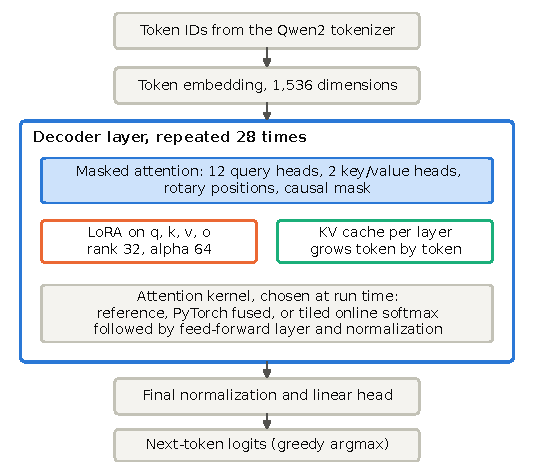
\includegraphics[width=\columnwidth]{model}
\caption{Qwen2.5-1.5B as used here. LoRA is attached to the four attention projections, the cache is read and written explicitly by my decoders, and the attention kernel can be swapped at run time.}
\label{fig:model}
\end{figure}

\subsection{System Pipeline}

Fig.~\ref{fig:pipeline} shows the whole system. The top row is the offline path on Kaggle, the middle row is what happens to one criterion in the live app, and the bottom row is the sequence of screens a user walks through. The same prompt format and the same output verifier are used in training, evaluation and the app, so the numbers I report describe the code that actually runs.

\begin{figure*}[t]
\centering
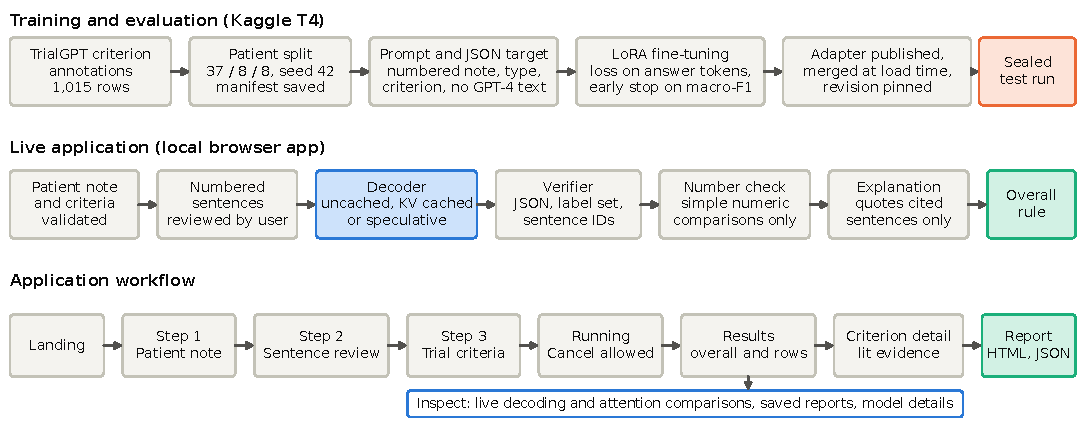
\includegraphics[width=\textwidth]{pipeline}
\caption{System pipeline and application workflow. Training and the sealed test evaluation ran on Kaggle, and the application runs locally in a browser.}
\label{fig:pipeline}
\end{figure*}

\subsection{Preprocessing and Output Schema}

A prompt contains the numbered patient note, the criterion type, the criterion text, plain definitions of the four allowed labels and the required answer format. The target is one JSON object, for example \texttt{\{"label": "included", "evidence": [0, 2]\}}, with sentence IDs preserved from the dataset. The prompts were tokenized with Qwen's chat template and nothing was truncated, because the longest prompts are 634 tokens in training, 468 in validation and 512 in test against a 32,768 token context window. A verifier parses each output, checks the label against the set allowed for that criterion type and drops any sentence ID that doesn't exist. Anything that can't be parsed is counted as wrong.

I don't train the model to write explanations. The dataset's only written explanations come from GPT-4, and when I tried having the base model explain verdicts it invented facts, calling a woman male and claiming that 58 falls outside a 25 to 65 age range. Explanations now use fixed wording that quotes the cited sentences exactly, which reads less smoothly but can't introduce a fact.

\subsection{Fine-Tuning}

LoRA replaces each frozen projection $W$ with
\begin{equation}
W' = W + \frac{\alpha}{r}\, B A,
\end{equation}
where $A$ and $B$ are trainable matrices of rank $r$ \cite{hu2022lora}. I applied it to the query, key, value and output projections of every layer. At $r=32$ and $\alpha=64$ that's 8,716,288 trainable parameters, about 0.56\% of the model. The loss is cross-entropy over the answer tokens only, with prompt positions masked out.

Training used AdamW at a learning rate of $2\times10^{-4}$, a 10\% linear warm-up, gradient clipping at 1.0, LoRA dropout of 0.05, batches of 4 with 2 accumulation steps, half-precision autocast and seed 42. Early stopping looked at generated validation macro-F1 with a patience of 2, breaking ties on evidence F1, since validation loss and macro-F1 didn't move together. Rare labels were optionally oversampled with weights proportional to $\mathrm{count}^{-p}$. Gradient checkpointing went in after a two-example laptop run hit 8.38 GB because of the autograd graph; with it the same run dropped to 5.2 GB and from 264 to 74 seconds, because it stopped paging. The adapter is merged into the weights when loaded for inference.

\subsection{KV-Cached Decoding}

Algorithm~\ref{alg:cache} is the decoder I wrote against the model's forward pass, using an explicit \texttt{DynamicCache}. Three things have to stay consistent once only the newest token is sent. The attention mask must still cover every cached token, because the library sizes the causal mask from the cache length plus the new tokens. The position ID must be the token's true position, or the rotary embedding would rotate it wrongly. The cache must be exactly one token longer after each step, which I assert every time. Memory grows linearly: each token costs layers $\times\,2\times$ KV heads $\times$ head width $\times$ 2 bytes, or $28\times2\times2\times128\times2 \approx 28.7$ KB here, which is why a 1,024 token prompt needs just 28 MB. Cached and uncached runs can differ slightly in their floating-point values because the matrix products are grouped differently, and tokens could only change if the top two logits were almost tied.

\begin{algorithm}[t]
\caption{Greedy decoding with an explicit KV cache}
\label{alg:cache}
\footnotesize
\begin{algorithmic}[1]
\Require prompt $x$, mask $m$, limit $T$
\State $C \gets$ empty cache; $p \gets$ positions from $m$
\State $\ell \gets \textsc{Forward}(x, m, p, C)$ \Comment{prefill}
\State $y \gets \arg\max \ell_{\text{last}}$
\While{$y$ is not EOS and fewer than $T$ tokens exist}
  \State append $y$ to output; $m \gets [m, 1]$; $p \gets p_{\text{last}} + 1$
  \State $\ell \gets \textsc{Forward}(y, m, p, C)$ \Comment{only the new token}
  \State assert $C$ grew by exactly one; $y \gets \arg\max \ell_{\text{last}}$
\EndWhile
\end{algorithmic}
\end{algorithm}

\subsection{Tiled Attention with Online Softmax}

The reference computes scaled dot-product attention \cite{vaswani2017attention},
\begin{equation}
O = \mathrm{softmax}\!\left(\frac{Q K^{\top}}{\sqrt{d}}\right) V,
\end{equation}
which needs the whole score matrix in memory at once. Algorithm~\ref{alg:tiled} splits queries and keys into tiles and keeps three running values for each query row: the largest score $m$, the normalizer $l$ and the partial output $O$. When a new tile raises the maximum from $m$ to $m'$, the older terms were measured against the old maximum, so
\begin{align}
l' &= e^{m-m'}\, l + \sum_j e^{s_j-m'},\\
O' &= e^{m-m'}\, O + \sum_j e^{s_j-m'}\, V_j,
\end{align}
and the row's final output is $O/l$ \cite{milakov2018online,dao2022flashattention}. Tiles that the causal mask covers completely are skipped without computing scores. No backend attention kernel is called, and the function can be patched into the real model in place of the library's.

\begin{algorithm}[t]
\caption{Tiled attention with online softmax}
\label{alg:tiled}
\footnotesize
\begin{algorithmic}[1]
\Require $Q, K, V$, causal mask $M$, tile sizes
\For{each query tile $q$}
  \State $m \gets -\infty$; $l \gets 0$; $O \gets 0$ for each row in $q$
  \For{each key tile $k$}
    \If{$M_{q,k}$ is fully masked} \textbf{continue} \EndIf
    \State $s \gets Q_q K_k^{\top}/\sqrt{d}$, fill masked positions with $-\infty$
    \State $m' \gets \max(m, \max_j s_j)$; $r \gets e^{m-m'}$
    \State $l \gets r\,l + \sum_j e^{s_j-m'}$
    \State $O \gets r\,O + \sum_j e^{s_j-m'} V_{k,j}$; $m \gets m'$
  \EndFor
  \State emit $O / l$
\EndFor
\end{algorithmic}
\end{algorithm}

\subsection{Greedy Speculative Decoding}

Qwen2.5-0.5B drafts and Qwen2.5-1.5B verifies, and the fine-tuned draft (rank 32, 4,325,376 trainable parameters) was trained on the same split. The pair peaks at about 2.89 and 0.94 GB, which nearly fills a 4 GB card, so the laptop app keeps the draft on the CPU by default, while Kaggle's benchmarks run both on the GPU. Both models use the same greedy settings as every other decoder here. Algorithm~\ref{alg:spec} shows one round. The invariant checked after every round is that both caches hold every token of the sequence except the last, which is the one both models still need to read. A rejection crops both caches back to the accepted tokens, and when every candidate is accepted the target's last prediction is a free bonus token, which the draft then has to read so it stays in step.

\begin{algorithm}[t]
\caption{One round of greedy speculative decoding}
\label{alg:spec}
\footnotesize
\begin{algorithmic}[1]
\Require sequence $S$, draft length $k$, caches $C_t, C_d$
\State $c \gets k$ greedy tokens from the draft, updating $C_d$
\State $\hat{y} \gets$ target's argmax at each position of $[S_{\text{last}}, c]$
\State $a \gets$ length of the longest prefix with $\hat{y}_i = c_i$
\State new tokens $\gets c_{1:a}$
\If{$a < |c|$} append correction $\hat{y}_{a+1}$
\Else{} append bonus token $\hat{y}_{|c|+1}$
\EndIf
\State extend $S$; crop $C_t$ and $C_d$ to $|S|-1$
\State feed the draft any token it hasn't read; assert both lengths
\end{algorithmic}
\end{algorithm}

\subsection{Evidence, Number Check and Overall Result}

Each result carries the criterion, label, cited sentence IDs, the exact evidence text and an explanation. The overall outcome is an aggregation rule applied to criterion predictions and isn't a ground-truth patient label. A patient is \emph{likely ineligible} only if a criterion failed with cited evidence, \emph{needs review} if anything is unknown, unverified or uncited, and \emph{potentially eligible} otherwise. Absent evidence never counts as proof in either direction, so an uncited verdict is shown as unconfirmed.

To get a bit more out of the system I added a deterministic number check on top of the model in the application. When a criterion is a bare numeric comparison and the note holds one clear value, plain code does the comparison and replaces a disagreeing verdict, and the row says so. It stays silent on anything less clear-cut. All test metrics in this paper are for the model alone, and the check was never run on the test split.

\subsection{Application}

The application is a FastAPI server with a React interface, started by double-clicking \texttt{start\_app.bat} after a one-time \texttt{setup\_app.bat}, so nobody needs a notebook, IDE or terminal to use it. A user pastes or uploads a note, repairs the numbered sentences if needed, enters criteria or imports them from ClinicalTrials.gov, and picks a decoding mode. Invalid input gets a plain message and work survives a page refresh. Fig.~\ref{fig:screens} shows the main screens. Results links each verdict to its highlighted sentences, reports download as HTML or JSON with the prototype notice and the exact model and adapter revisions, and Inspect runs real decoding and attention comparisons on demand rather than showing stored charts.

\begin{figure*}[t]
\centering
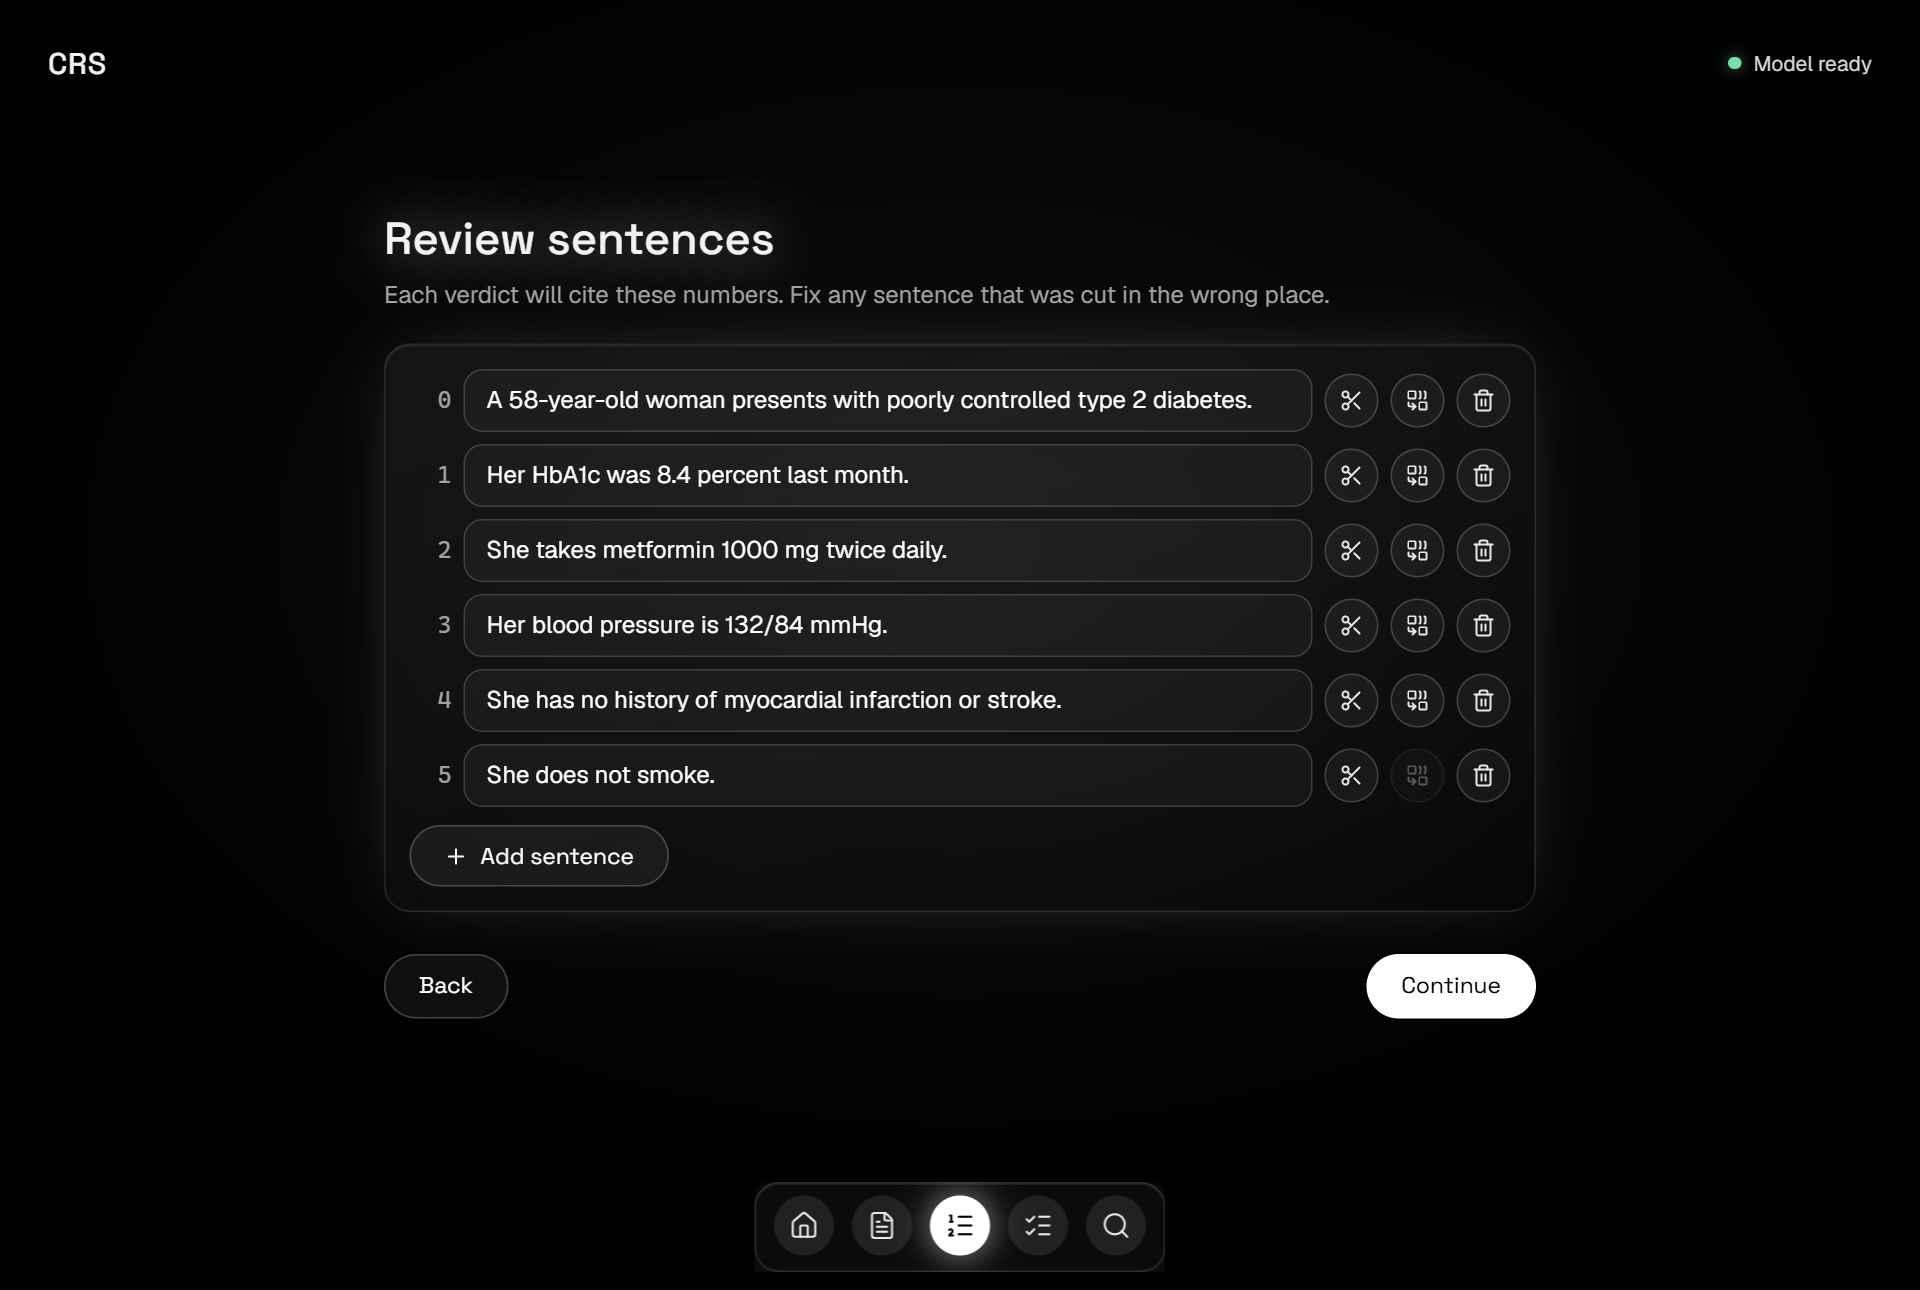
\includegraphics[width=0.49\textwidth]{app_sentences.png}\hfill
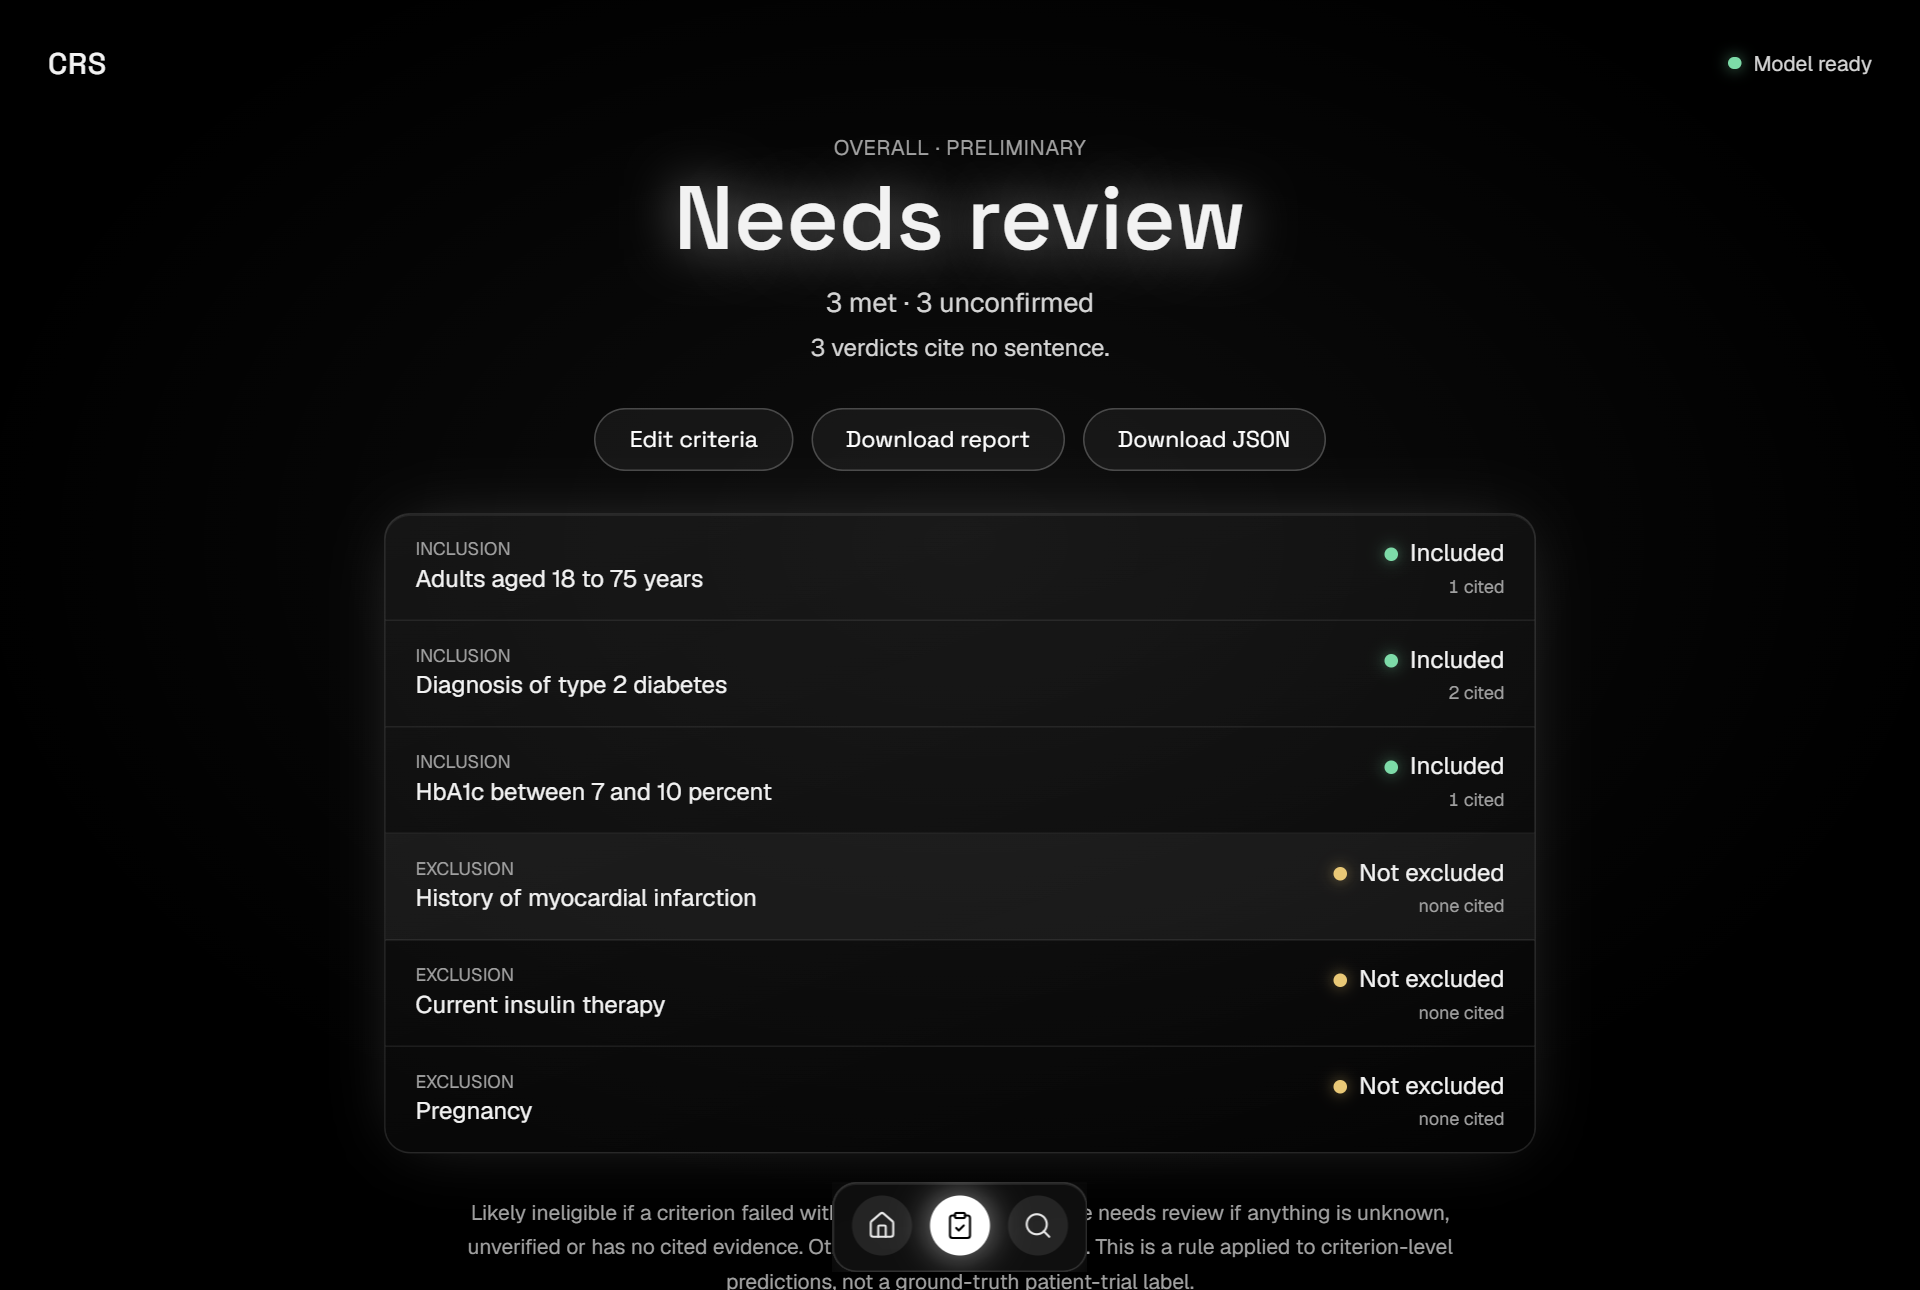
\includegraphics[width=0.49\textwidth]{app_results.png}\\[4pt]
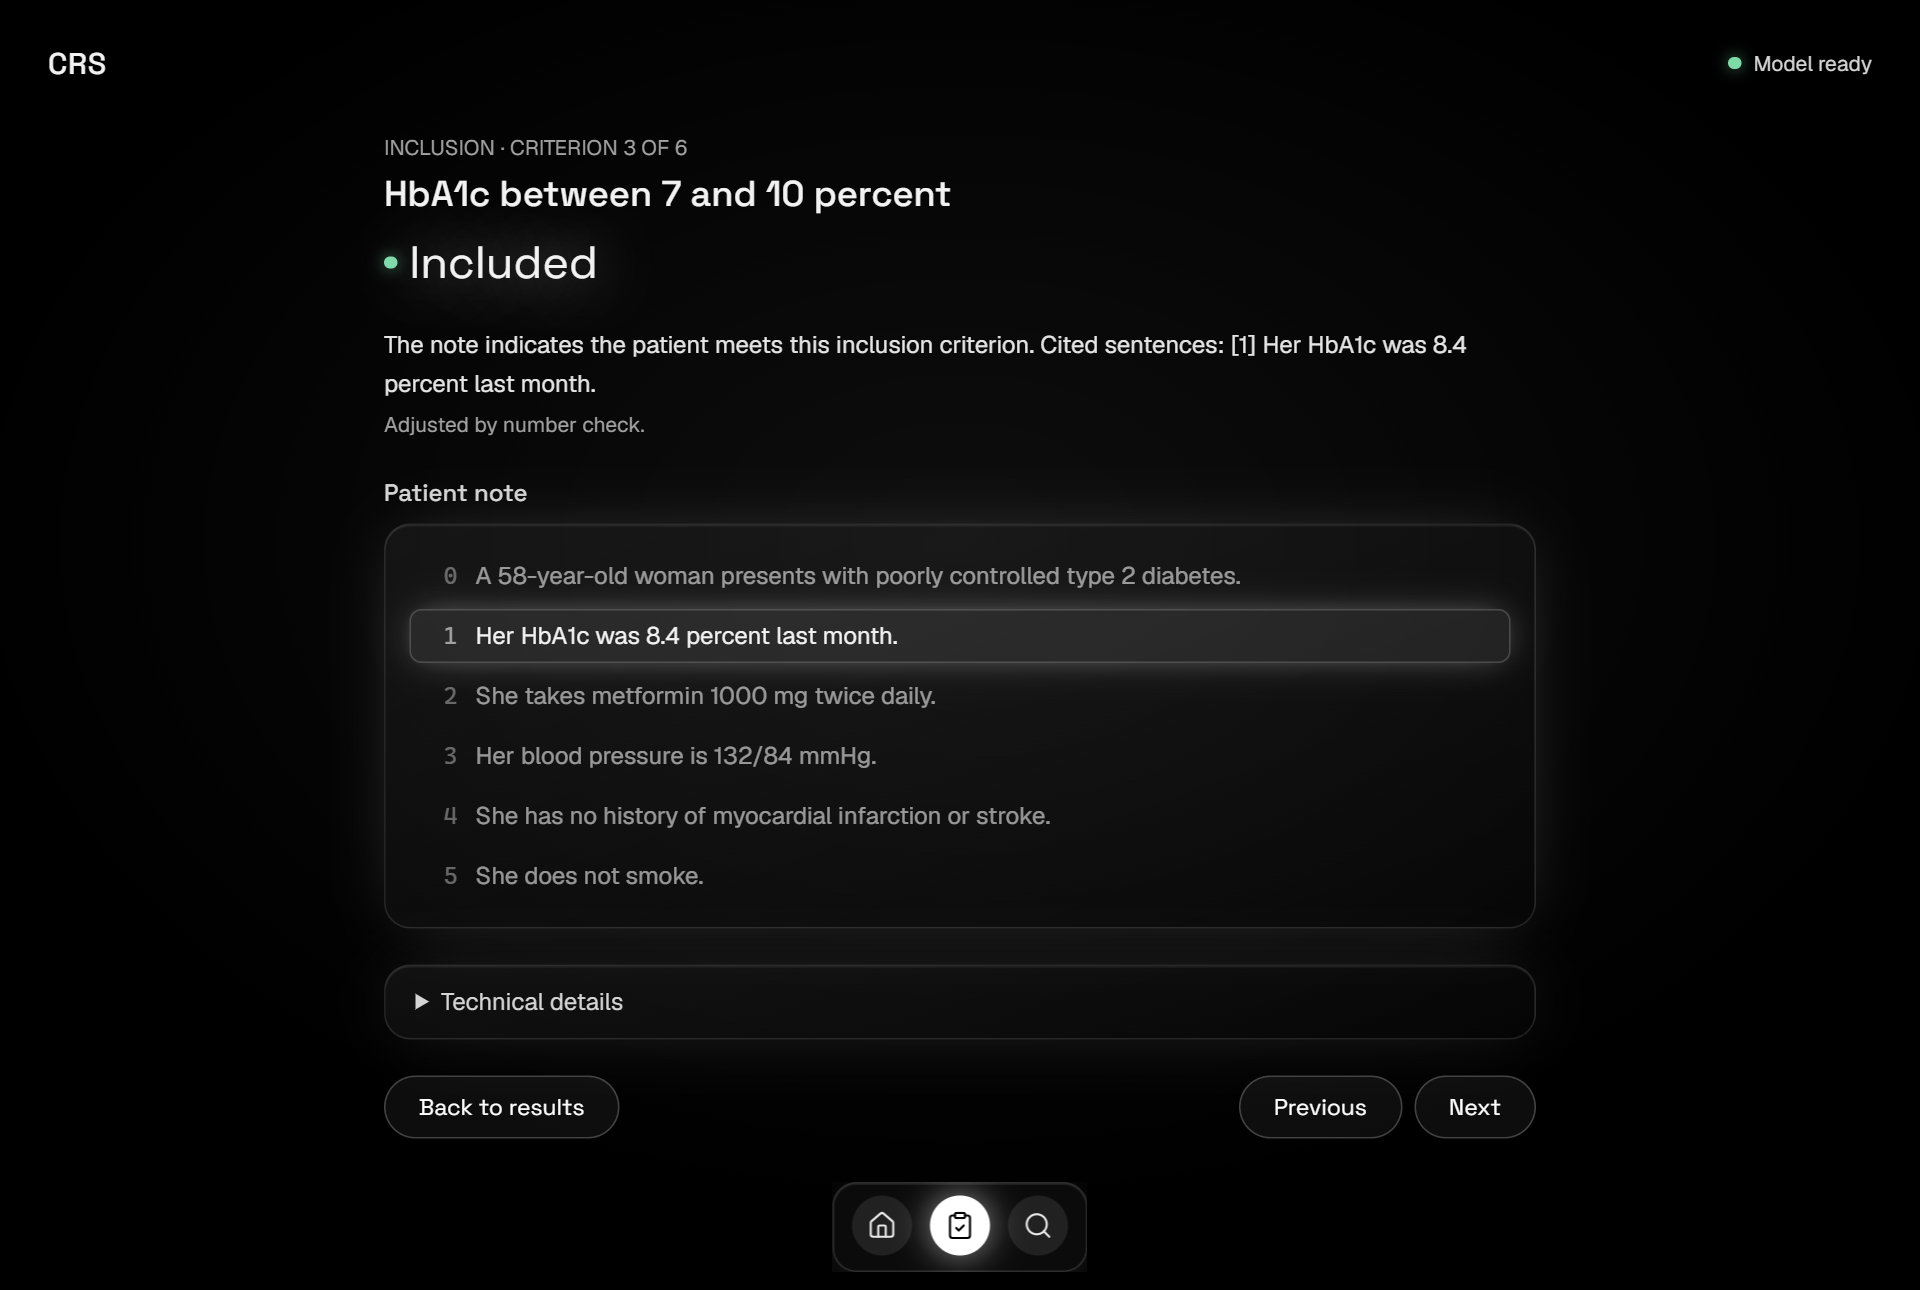
\includegraphics[width=0.49\textwidth]{app_detail.png}\hfill
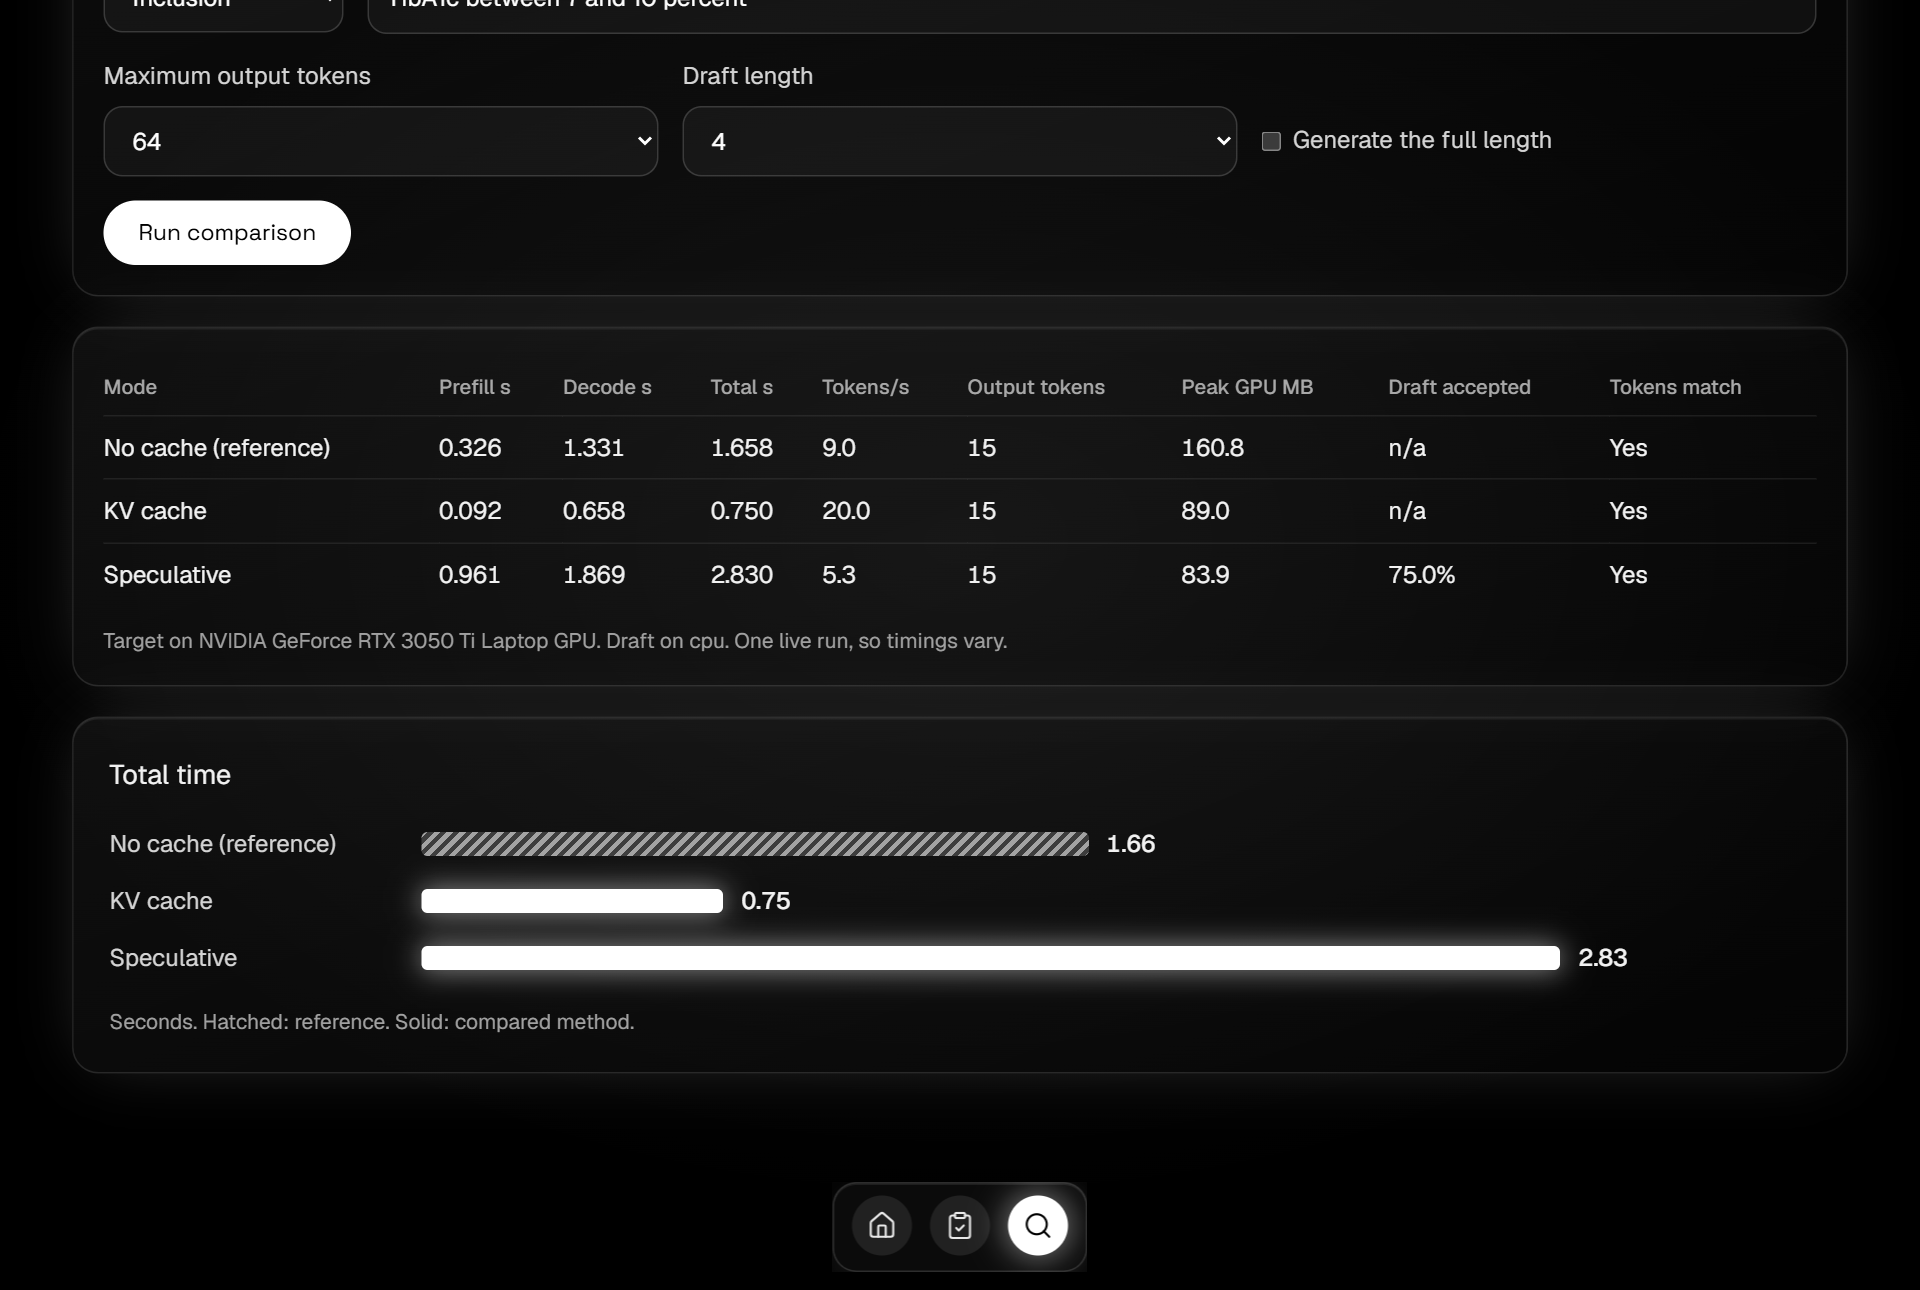
\includegraphics[width=0.49\textwidth]{app_inspect.png}
\caption{The application: sentence review (top left), results with counts and the reason for the outcome (top right), a criterion with its evidence highlighted (bottom left), and the live decoding comparison in Inspect (bottom right).}
\label{fig:screens}
\end{figure*}

\section{Experimental Setup and Metrics}

Training, the final evaluation and the benchmarks in the tables below ran on one NVIDIA Tesla T4 on Kaggle, from a frozen commit tagged \texttt{final-config}, with PyTorch 2.11 and Transformers 5.8. I also ran the benchmarks on the laptop's RTX 3050 Ti. All evaluation uses deterministic greedy decoding with sampling off, one beam, a repetition penalty of 1.0 and at most 96 new tokens, because Qwen's bundled defaults turn on sampling and a repetition penalty. The test split could only be read with an explicit flag and every access was logged.

Classification is scored with accuracy, macro-F1, per-class precision, recall and F1, and confusion matrices, overall and separately for inclusion and exclusion. A label absent from the gold set of a split is left out of macro-F1 and marked n/a, and I also report the score with it counted as zero. An invalid output counts as wrong. Evidence is scored as micro precision, recall and F1, and as macro F1 two ways. Over all rows, a row where both sets are empty scores 1 and one where only one is empty scores 0, while the second macro uses only rows with gold evidence. Uncertainty comes from a patient-level bootstrap with 2,000 resamples, since rows from one patient aren't independent.

Each benchmark discards warm-up runs, synchronizes the GPU around its timers, and reports the median of 5 repeats. Output length is fixed by ignoring EOS in the cache benchmark.

\section{Results and Discussion}

\subsection{Fine-Tuning and Model Selection}

Table~\ref{tab:runs} lists every run, all judged on validation only. R3 was chosen by the rule fixed in advance: highest macro-F1, then evidence F1, among the Qwen 1.5B runs. The gaps among R1, R2 and R3 are small, and with a patient-level interval of 0.42 to 0.64 they may well be noise, so I wouldn't claim R3 is clearly the best setting. Putting evidence before the label (R4) raised evidence F1 slightly but cost 0.10 of macro-F1, so I kept the label first.

\begin{table}[t]
\caption{Validation Results by Run (206 Rows)}
\label{tab:runs}
\centering
\footnotesize
\setlength{\tabcolsep}{3pt}
\begin{tabular}{@{}llrrcrrrr@{}}
\toprule
Run & Model & $r$ & $p$ & Ord. & Ep. & Acc. & M-F1 & Ev-F1 \\
\midrule
R0 & Qwen 1.5B & -- & -- & -- & -- & 0.175 & 0.147 & 0.106 \\
R0b & SmolLM2 1.7B & -- & -- & -- & -- & 0.180 & 0.120 & 0.111 \\
R1 & Qwen 1.5B & 16 & 0.0 & L & 3 & 0.752 & 0.534 & 0.462 \\
R2 & Qwen 1.5B & 16 & 0.5 & L & 4 & 0.738 & 0.552 & 0.486 \\
\textbf{R3} & \textbf{Qwen 1.5B} & \textbf{32} & \textbf{0.5} & \textbf{L} & \textbf{4} & \textbf{0.743} & \textbf{0.558} & \textbf{0.509} \\
R4 & Qwen 1.5B & 32 & 0.5 & E & 7 & 0.762 & 0.459 & 0.526 \\
R5 & SmolLM2 1.7B & 32 & 0.5 & L & 2 & 0.675 & 0.514 & 0.446 \\
R6 & Qwen 0.5B & 32 & 0.5 & L & 2 & 0.738 & 0.446 & 0.491 \\
\bottomrule

\end{tabular}

\vspace{2pt}
\raggedright\scriptsize $r$: LoRA rank, $p$: oversampling power, Ord.: L is label first, E is evidence first, Ep.: best epoch. R0 and R0b are untrained.
\end{table}

Fig.~\ref{fig:training} shows R3's training. Training loss falls steadily while validation loss stops improving after epoch 3, which is the overfitting I'd expect from 602 rows. The small dataset makes more parameters or more epochs a poor idea, so early stopping kept epoch 4 and discarded the rest. The epoch-to-epoch swings in macro-F1 also show how much two or three rare-label rows can move this metric.

\begin{figure}[t]
\centering
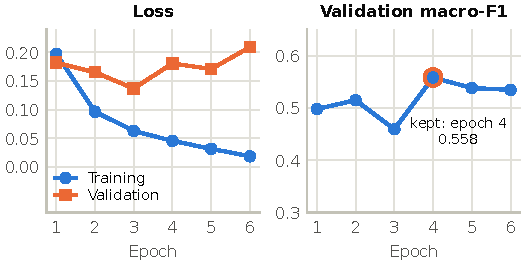
\includegraphics[width=\columnwidth]{training}
\caption{Training curves for the selected run R3. The model from epoch 4 was kept and training stopped at epoch 6.}
\label{fig:training}
\end{figure}

\subsection{Held-Out Classification}

Table~\ref{tab:eval} and Fig.~\ref{fig:before_after} compare the same model before and after fine-tuning on identical rows with identical decoding settings. On test, accuracy rose from 0.204 to 0.728 and macro-F1 from 0.234 to 0.560. The majority baseline's accuracy of 0.626 shows how far a trivial rule gets on skewed data, but its macro-F1 of 0.272 exposes that it learns nothing about rare labels. The test macro-F1 is close to validation's 0.558, so selecting on validation didn't flatter the model noticeably. With \emph{excluded} counted as zero rather than left out, test macro-F1 is 0.466. The bootstrap intervals are wide, 0.60 to 0.83 for accuracy and 0.43 to 0.64 for macro-F1, because there are only 8 test patients.

\begin{table}[t]
\caption{Before and After Fine-Tuning, Accuracy and Macro-F1}
\label{tab:eval}
\centering
\footnotesize
\setlength{\tabcolsep}{3.5pt}
\begin{tabular}{@{}llrrrrrr@{}}
\toprule
 & & \multicolumn{2}{c}{Untrained} & \multicolumn{2}{c}{Baseline} & \multicolumn{2}{c}{Fine-tuned} \\
Split & Group & Acc. & M-F1 & Acc. & M-F1 & Acc. & M-F1 \\
\midrule
Test & Overall & 0.204 & 0.234 & 0.626 & 0.272 & 0.728 & 0.560 \\
 & Inclusion & 0.267 & 0.203 & 0.507 & 0.168 & 0.773 & 0.469 \\
 & Exclusion & 0.168 & 0.170 & 0.695 & 0.273 & 0.702 & 0.427 \\
\midrule
Validation & Overall & 0.175 & 0.147 & 0.621 & 0.215 & 0.743 & 0.558 \\
 & Inclusion & 0.197 & 0.126 & 0.409 & 0.145 & 0.727 & 0.379 \\
 & Exclusion & 0.164 & 0.112 & 0.721 & 0.210 & 0.750 & 0.574 \\
\bottomrule

\end{tabular}
\end{table}

\begin{figure}[t]
\centering
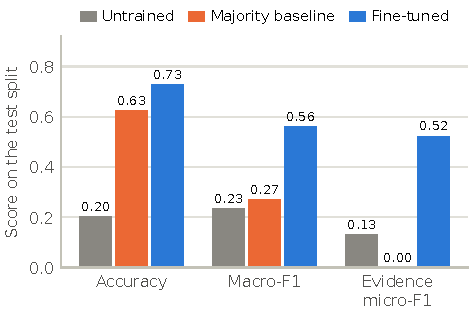
\includegraphics[width=\columnwidth]{before_after}
\caption{Test scores for the untrained model, the majority baseline and the fine-tuned model. The baseline cites nothing, so its evidence micro-F1 is zero.}
\label{fig:before_after}
\end{figure}

The per-class results in Table~\ref{tab:perclass}, given overall and separately for each criterion type, and the confusion matrices in Fig.~\ref{fig:confusion} show where the errors sit. Every time the model said \emph{included} it was right (precision 1.000), and it catches 95.6\% of \emph{not excluded} rows, but it finds only 1 of 7 \emph{not included} rows. Two habits explain most of the 56 mistakes. On exclusion criteria it defaults to \emph{not excluded}, which accounts for 32 errors, and 24 of those should have been \emph{not enough information}. On inclusion criteria it retreats to \emph{not enough information} whenever the answer needs a clinical inference, which is why that label has perfect recall on inclusion rows.

\begin{table}[t]
\caption{Per-Class Scores of the Fine-Tuned Model on Test}
\label{tab:perclass}
\centering
\footnotesize
\setlength{\tabcolsep}{4pt}
\begin{tabular}{@{}llrrrr@{}}
\toprule
Group & Label & Support & Precision & Recall & F1 \\
\midrule
Overall & Included & 27 & 1.000 & 0.704 & 0.826 \\
 & Not included & 7 & 0.500 & 0.143 & 0.222 \\
 & Not excluded & 91 & 0.731 & 0.956 & 0.829 \\
 & Excluded & 0 & -- & -- & -- \\
 & Not enough information & 66 & 0.667 & 0.606 & 0.635 \\
 & Not applicable & 15 & 0.500 & 0.200 & 0.286 \\
\midrule
Inclusion & Included & 27 & 1.000 & 0.704 & 0.826 \\
 & Not included & 7 & 0.500 & 0.143 & 0.222 \\
 & Not enough information & 38 & 0.704 & 1.000 & 0.826 \\
 & Not applicable & 3 & 0.000 & 0.000 & 0.000 \\
\midrule
Exclusion & Not excluded & 91 & 0.731 & 0.956 & 0.829 \\
 & Excluded & 0 & -- & -- & -- \\
 & Not enough information & 28 & 0.333 & 0.071 & 0.118 \\
 & Not applicable & 12 & 0.500 & 0.250 & 0.333 \\
\bottomrule

\end{tabular}
\end{table}

\begin{figure*}[t]
\centering
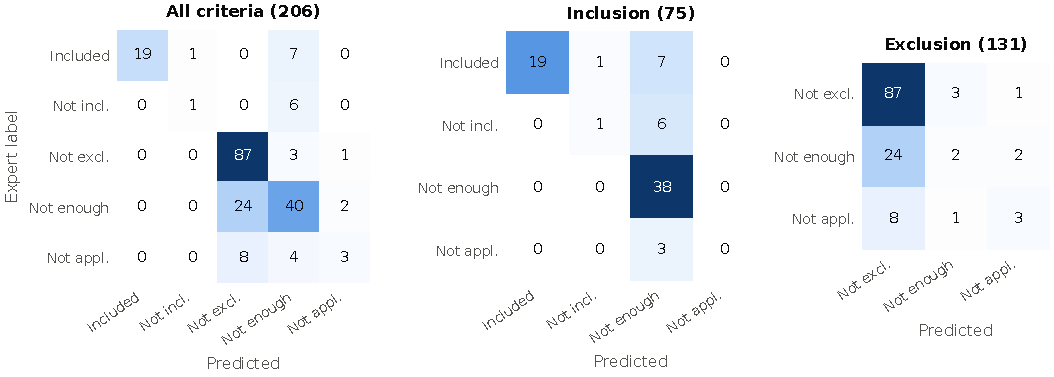
\includegraphics[width=\textwidth]{confusion}
\caption{Test confusion matrices for the fine-tuned model, with expert labels in rows. \emph{Excluded} is omitted because it has no test rows and the model never predicted it, and no output was invalid.}
\label{fig:confusion}
\end{figure*}

\subsection{Evidence Retrieval}

Table~\ref{tab:evidence} reports evidence quality. Fine-tuning raised micro-F1 from 0.130 to 0.523, mostly by making the model stop citing sentences at random: rows where gold evidence is empty but the model cites something fell from 82 to 9. The macro over all rows looks high at 0.817, but 136 of the 206 rows have two empty sets and score a free 1, so the 0.528 over rows with gold evidence is the fairer figure. Exclusion evidence is weak at a micro-F1 of 0.190 and a recall of 0.125, which fits how the model was taught, since 74.7\% of training \emph{not excluded} rows have no evidence.

\begin{table}[t]
\caption{Evidence Sentence Retrieval on Test}
\label{tab:evidence}
\centering
\footnotesize
\setlength{\tabcolsep}{4pt}
\begin{tabular}{@{}llrrrrr@{}}
\toprule
 & & \multicolumn{3}{c}{Micro} & \multicolumn{2}{c}{Macro F1} \\
Model & Group & P & R & F1 & All & Gold \\
\midrule
Untrained & Overall & 0.078 & 0.394 & 0.130 & 0.358 & 0.176 \\
 & Inclusion & 0.226 & 0.306 & 0.260 & 0.442 & 0.136 \\
 & Exclusion & 0.046 & 0.562 & 0.085 & 0.310 & 0.287 \\
\midrule
Fine-tuned & Overall & 0.577 & 0.479 & 0.523 & 0.817 & 0.528 \\
 & Inclusion & 0.603 & 0.661 & 0.631 & 0.690 & 0.638 \\
 & Exclusion & 0.400 & 0.125 & 0.190 & 0.889 & 0.219 \\
\bottomrule

\end{tabular}
\end{table}

\subsection{Error Analysis}

Table~\ref{tab:errors} lists twelve test cases that I read against their notes, and the full write-up is in \texttt{results/error\_analysis.md}. The causes are my own reading and haven't been reviewed by a clinician. Cases 3 to 5 show the model finding the right sentence and refusing to conclude, while cases 7 and 8 show that a correct label or a valid sentence ID doesn't guarantee relevant evidence. Case 10 is the most interesting one for the dataset itself: two near-identical pregnancy criteria on male patients have different expert labels, so part of the weak \emph{not applicable} score (F1 0.286) reflects a boundary the annotations don't draw consistently. No output was invalid in the 412 validation and test rows, so the verifier's handling of bad JSON is covered only by unit tests. No test note held a true contradiction either, which makes case 12 the closest I can show.

\begin{table*}[t]
\caption{Representative Errors on the Test Split}
\label{tab:errors}
\centering
\footnotesize
\begin{tabular}{@{}rrp{4.3cm}p{2.2cm}p{2.2cm}p{5.6cm}@{}}
\toprule
\# & ID & Criterion (type) & Gold, evidence & Predicted, evidence & Likely cause \\
\midrule
1 & 176 & No history of central venous catheterization (inc.) & included, [0] & not included, [] & Polarity flip on a negated criterion, near match with an arterial catheter \\
2 & 403 & Positive hepatitis B, C or HIV screening (exc.) & not enough info., [] & not excluded, [] & Missing information treated as a no \\
3 & 186 & Heart rate of at least 90/min (inc.) & included, [2] & not enough info., [2] & Note says tachycardic with no number, inference not made \\
4 & 195 & Pain at least 3 out of 10 (inc.) & included, [0] & not enough info., [0] & ``Excruciating'' not mapped to a numeric scale \\
5 & 185 & Diagnosed with shock or ARDS (inc.) & included, [2, 3] & not enough info., [] & Shock must be inferred from blood pressure 80/60 \\
6 & 382 & At least 4 ACR criteria for SLE (inc.) & included, [0, 1, 2] & not enough info., [0--3] & Abbreviation and counting; the spelled-out form (413) was accepted \\
7 & 416 & Referred from ED for suspected appendicitis (inc.) & included, [0, 5] & included, [0, 1, 3] & Right label, an irrelevant citation and the ultrasound missed \\
8 & 832 & Symptom score no greater than 6 (inc.) & not enough info., [] & not enough info., [0--7] & Unsupported blanket citation, no score in the note \\
9 & 414 & Patients without SLE (exc.) & not excluded, [0--3] & not excluded, [] & Right label, evidence omitted \\
10 & 697, 322 & Pregnancy criteria on male patients (exc.) & n/a, [] and not excl., [0] & not excl., [] and n/a, [] & Expert labels differ for the same situation \\
11 & 836 & Wheezing history after age 6 (inc.) & not included, [0, 1] & not enough info., [1] & Temporal reasoning: the patient is 4 years old \\
12 & 827 & Clinical diagnosis of asthma (inc.) & not enough info., [0--3, 6] & not enough info., [1, 3, 4] & Apparent conflict of no history of wheezing with current wheezing \\
\bottomrule
\end{tabular}
\end{table*}

When I rehearsed the finished app on five invented notes, the model matched 14 of my 24 expected labels, and comparing numbers was the clearest weakness: with a BMI of 33 it answered that ``BMI of at least 30'' wasn't met. That's why I built the number check. I developed it on training notes only and judged it once on validation against a bar set in advance, that every decision had to match the expert label. It made 5 decisions and all 5 were right, but they were all age criteria the model already had right, so it changed nothing on validation and BMI and laboratory values remain unmeasured on the dataset. With the check and a cleanup of note headings the rehearsal rose to 18 of 24, though that isn't independent evidence because I built the check after seeing those failures.

\subsection{KV-Cached Decoding}

Generated tokens were identical to the uncached reference in all 9 input and output combinations in Table~\ref{tab:cache}, and the largest logit difference was 0.168, small enough never to change a token. Fig.~\ref{fig:cache} shows the speedup growing with prompt length, from between 1.1 and 1.45 times at 64 input tokens to 8.97 times at 1,024 input and 256 output tokens, because an uncached step reprocesses the whole sequence while a cached step costs the same at any length. Cached decode steps held about 25 tokens per second throughout, and uncached decoding fell to 2.8. The prefill costs the same in both, so the cache only pays off once decoding starts. Peak memory above the model was also lower with the cache, 346 MB against 745 MB in the largest case, since the uncached path keeps rebuilding activations for the full sequence.

\begin{table*}[t]
\caption{KV-Cached Versus Uncached Greedy Decoding on the T4 (Fine-Tuned 1.5B, Half Precision, Median of 5)}
\label{tab:cache}
\centering
\footnotesize
\begin{tabular}{@{}rrrrrrrrrr@{}}
\toprule
 & & & \multicolumn{2}{c}{Decode (s)} & \multicolumn{2}{c}{Tokens per second} & \multicolumn{2}{c}{Peak above model (MB)} & \\
Input & Output & Prefill (s) & Uncached & Cached & Uncached & Cached & Uncached & Cached & Speedup \\
\midrule
64 & 16 & 0.044 & 0.64 & 0.57 & 23.6 & 26.1 & 46 & 22 & 1.11$\times$ \\
64 & 64 & 0.045 & 2.73 & 2.46 & 23.1 & 25.6 & 74 & 22 & 1.11$\times$ \\
64 & 256 & 0.048 & 14.38 & 9.91 & 17.7 & 25.7 & 186 & 22 & 1.45$\times$ \\
256 & 16 & 0.056 & 1.18 & 0.59 & 13.1 & 24.9 & 158 & 87 & 1.91$\times$ \\
256 & 64 & 0.051 & 5.06 & 2.43 & 12.5 & 25.8 & 186 & 87 & 2.06$\times$ \\
256 & 256 & 0.051 & 24.88 & 9.94 & 10.3 & 25.6 & 298 & 87 & 2.49$\times$ \\
1024 & 16 & 0.286 & 4.78 & 0.60 & 3.2 & 18.2 & 606 & 346 & 5.74$\times$ \\
1024 & 64 & 0.290 & 20.59 & 2.44 & 3.1 & 23.4 & 634 & 346 & 7.63$\times$ \\
1024 & 256 & 0.295 & 92.40 & 10.03 & 2.8 & 24.8 & 745 & 346 & 8.97$\times$ \\
\bottomrule

\end{tabular}
\end{table*}

\begin{figure}[t]
\centering
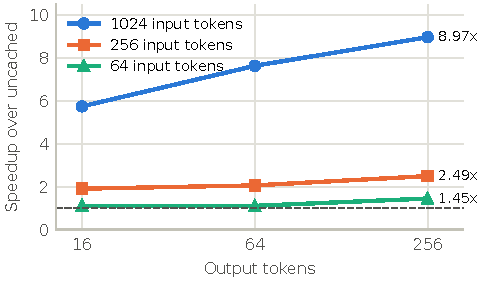
\includegraphics[width=\columnwidth]{cache}
\caption{Speedup of cached over uncached decoding. The dashed line marks no speedup.}
\label{fig:cache}
\end{figure}

\subsection{Tiled Attention}

Across shapes and causal masks, tiled attention agreed with the reference to a maximum absolute error of $1.3\times10^{-6}$ in single precision and a mean error below $6\times10^{-8}$, as Table~\ref{tab:attention} shows. Its memory use is the clear win. At length 4096 the reference needed 1,536 MB of GPU memory above its inputs while 256-token tiles needed 18.5 MB, a factor of 83, because the full score matrix never exists. About half the tiles are skipped by the causal mask (120 of 256 at that size).

\begin{table*}[t]
\caption{Attention Runtime, Memory and Numerical Error on the T4 GPU (8 Heads, Causal Mask, Single Precision, Median of 5)}
\label{tab:attention}
\centering
\footnotesize
\begin{tabular}{@{}rrrrrrrrr@{}}
\toprule
 & \multicolumn{4}{c}{Median runtime (ms)} & \multicolumn{2}{c}{Peak above inputs (MB)} & \multicolumn{2}{c}{Worst error, all tile sizes} \\
Length & Reference & PyTorch fused & Tiled 64 & Tiled 256 & Reference & Tiled 256 & Maximum & Mean \\
\midrule
256 & 0.5 & 0.3 & 5.5 & 0.8 & 6.0 & 6.5 & 1.0e-6 & 4.2e-8 \\
1024 & 3.2 & 2.0 & 74.0 & 7.2 & 96.1 & 8.0 & 1.3e-6 & 3.2e-8 \\
4096 & 41.9 & 13.9 & 1040.7 & 87.9 & 1536.4 & 18.5 & 8.9e-7 & 2.6e-8 \\
\bottomrule

\end{tabular}
\end{table*}

The runtime in Fig.~\ref{fig:attention} is a different story, and it's what the theory predicts for an educational version. On the GPU every tiled setting is slower than the reference, and PyTorch's fused kernel beats everything, with 16-token tiles taking 16 seconds at length 4096 against 14 ms. Each tile costs Python interpreter time, separate GPU submissions and small allocations, while a compiled kernel runs the same loop with none of that \cite{dao2022flashattention}. Bigger tiles mean fewer of those overheads, which is why 256-token tiles come closest. On the T4 machine's CPU, 256-token tiles did beat the plain reference at length 4096 (390 ms against 2,032 ms), though the fused kernel was faster still at 276 ms.

\begin{figure}[t]
\centering
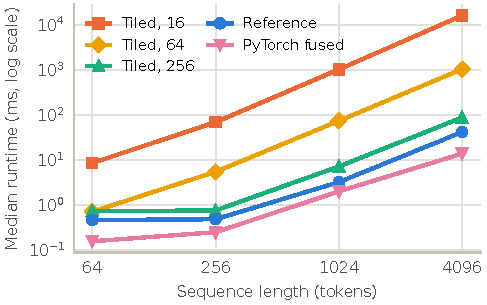
\includegraphics[width=\columnwidth]{attention}
\caption{Attention runtime on the T4 GPU for the reference, PyTorch's fused kernel and three tile sizes. Exact values are in Table~\ref{tab:attention}.}
\label{fig:attention}
\end{figure}

\subsection{Speculative Decoding}

Speculative decoding produced tokens identical to greedy decoding in every scenario and draft length, so the cache synchronization is correct, but as Fig.~\ref{fig:speculative} and Table~\ref{tab:speculative} show, it was slower everywhere on the T4, between 0.51 and 0.85 times greedy speed. Acceptance on real screening prompts was high with the fine-tuned draft, 90\% to 97\%, against 67\% to 85\% with the untrained draft, and that's why only the fine-tuned draft improves as $k$ grows on those prompts. The longer free-form generations accept less, and drafting more tokens then wastes more work.

\begin{table*}[t]
\caption{Speculative Decoding With the Fine-Tuned 0.5B Draft on the T4, Median of 5}
\label{tab:speculative}
\centering
\footnotesize
\begin{tabular}{@{}lrrrrrrrr@{}}
\toprule
Scenario & Greedy (s) & $k$ & Total (s) & Acceptance & Tokens per round & Tok/s & Peak above models (MB) & Relative speed \\
\midrule
Screening JSON & 12.04 & 2 & 15.83 & 0.971 & 2.74 & 18.2 & 117 & 0.76$\times$ \\
 &  & 4 & 14.90 & 0.909 & 4.24 & 19.3 & 117 & 0.81$\times$ \\
 &  & 8 & 14.23 & 0.901 & 6.40 & 20.2 & 117 & 0.85$\times$ \\
\midrule
256 in, 128 out & 5.03 & 2 & 6.55 & 0.748 & 2.46 & 19.5 & 84 & 0.77$\times$ \\
 &  & 4 & 7.11 & 0.592 & 3.37 & 18.0 & 84 & 0.71$\times$ \\
 &  & 8 & 9.12 & 0.433 & 4.41 & 14.0 & 84 & 0.55$\times$ \\
\midrule
1024 in, 128 out & 5.23 & 2 & 7.22 & 0.701 & 2.37 & 17.7 & 338 & 0.72$\times$ \\
 &  & 4 & 7.75 & 0.556 & 3.20 & 16.5 & 338 & 0.68$\times$ \\
 &  & 8 & 10.22 & 0.388 & 4.00 & 12.5 & 338 & 0.51$\times$ \\
\bottomrule

\end{tabular}
\end{table*}

\begin{figure}[t]
\centering
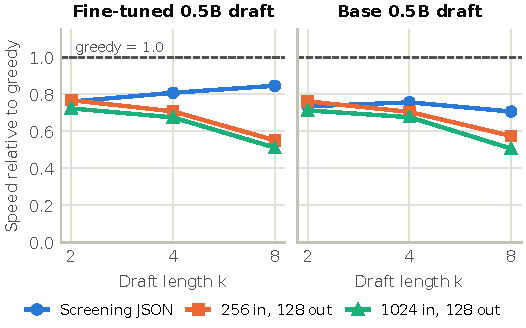
\includegraphics[width=\columnwidth]{speculative}
\caption{Speculative decoding speed relative to greedy on the T4. Every setting is below the dashed line at 1.0, and tokens matched greedy throughout.}
\label{fig:speculative}
\end{figure}

The reason is cost per step. Speculative decoding only helps if a draft step is much cheaper than a target step, and here a 0.5B step took about 24 ms against 39 ms for the 1.5B target, because interpreter time and mask building don't shrink with the model. For the screening workload at $k=2$, greedy took 12.04 s in total, while speculative spent 2.31 s prefilling two models, 6.92 s drafting, 3.89 s verifying and 2.72 s synchronizing caches. Outputs of about 14 tokens also leave little room to recover that overhead. The cited 2 to 3 times gains come from far larger targets \cite{leviathan2023fast,chen2023accelerating}. On the laptop, a CPU draft ran at 0.26 to 0.38 times greedy speed. A GPU draft ran at 0.36 to 0.54 times, apart from a 1.06 to 1.09 times result at 1,024 input tokens that I don't count as a real gain, since with both models loaded the 4 GB card was nearly full, which slowed greedy decoding itself. Tokens matched in all of these runs as well.

\subsection{Decisions and Failures}

Several results came from things going wrong. The first Kaggle training run crashed because the preinstalled torchao was too old for PEFT, so that package is now pinned. Writing explanations with the model was tried and dropped, as described earlier. Vercel was rejected for deployment because it has no GPU and can't keep a 3 GB model loaded. The final Kaggle session also timed out during the last benchmark and lost its files, so the notebook was rerun from the same commit, meaning the sealed test ran twice. Nothing changed between the two runs, the test numbers agreed to four decimal places, and both are in the access log. After the test split had been opened I considered retraining and a larger model, and rejected both: the first would have meant tuning against data I'd already seen, and added training data would break the single-dataset rule. In the app's first real double-click, the browser opened before the server was ready and the GPU ran out of memory once, so the browser now waits for the model and loading retries.

\section{Limitations}

The test split has 8 patients and 206 rows, so the intervals are wide and one annotator's habits on one long trial can move the totals: 17 of the 24 rows in the largest error group come from a single patient on one trial. The \emph{excluded} label has no test rows, and \emph{not included} has 7. Expert labels are themselves inconsistent in places. The model is small and unreliable at comparing numbers and at medical knowledge, for instance reading apixaban without connecting it to anticoagulant therapy. A cited verdict can still be wrong, because a citation shows where the model looked and doesn't prove its reasoning, which is why every verdict needs a person to check it. The number check handles only simple comparisons and has no validation evidence on BMI or laboratory values.

Timings differ between Kaggle and the laptop, and only 2 repeats were used for the laptop's speculative runs. The app's margin on a 4 GB GPU is thin, since about 3.2 GB is free and the model needs nearly all of it. Without a GPU the app still works, but six criteria take about 40 seconds with at least 8 GB of free memory and about 2 minutes with less. Finally, a model larger than 1.5B would likely do better on numbers and medical knowledge, but it wouldn't fit the local live-demonstration requirement on this hardware.

\section{Conclusion}

A 1.5B open-weight model tuned with LoRA on 602 expert rows reached 0.728 accuracy and 0.560 macro-F1 on held-out patients, well above both its untrained self and a majority baseline, and it runs live in a browser on a 4 GB laptop GPU. The hand-written cache gave up to 8.97 times faster decoding with identical tokens, and tiled attention matched the reference within about $10^{-6}$ using 83 times less memory, while speculative decoding worked correctly but didn't pay off at this scale. The main improvements left are more data for rare labels, a consistent annotation rule for \emph{not applicable}, letting the model show its working before answering, and a larger model on hardware that can serve it.

\section*{Reproducibility and Submission Materials}

Source, split manifest, benchmark logs and setup instructions are at \url{https://github.com/FaatehHaneef/Clinical-records-screener}. The adapters are at \url{https://huggingface.co/faa-tehe/crs-qwen2.5-1.5b-lora} and \url{https://huggingface.co/faa-tehe/crs-qwen2.5-0.5b-draft-lora}, with revisions pinned in \texttt{adapters.lock.json}. On Windows, run \texttt{setup\_app.bat} once and then \texttt{start\_app.bat}. Training and final evaluation are in the \texttt{kaggle/} notebooks, and every figure and results table here is generated from \texttt{results/} by \texttt{report/make\_assets.py}.

Demonstration video: \underline{\hspace{5.5cm}}

\section*{Appendix: Use of AI Assistance}

I used Claude Code (Anthropic) as an AI assistant during this project for writing and debugging code, setting up experiments, analyzing results and drafting this report. Off-the-shelf libraries include PyTorch, Transformers, PEFT, FastAPI and React, the interface adapts a dock component from 21st.dev and uses the thinking-orbs library, and the cached decoder, tiled attention and speculative decoder were written for this project rather than taken from a library. Reused and generated code was tested with an automated suite of 261 tests, and each reported number comes from logged runs in the repository.

\bibliographystyle{IEEEtran}
\bibliography{refs}

\end{document}
